\documentclass{if-beamer}

% --------------------------------------------------- %
%                  Presentation info	              %
% --------------------------------------------------- %
\title[$\tau$-cristais rígidos]{$\tau$-cristais rígidos}
\subtitle{Rigid $\tau$-crystals}
\author{Daniel Kawai \\ Douglas Smigly}
\institute[IME-USP]{
  Instituto de Matemática e Estatística\\
  Universidade de São Paulo
}
\date{\today}
\logo{

\includegraphics[scale=0.0165]{IME-logo.png}
}
\subject{Presentation subject} % metadata

\graphicspath{{figuras/}}
% --------------------------------------------------- %
%                    Title + Schedule                 %
% --------------------------------------------------- %

\begin{document}

\begin{frame}
  \titlepage
\end{frame}

\begin{frame}{Conteúdo}
  \tableofcontents
\end{frame}

% --------------------------------------------------- %
%                      Presentation                   %
% --------------------------------------------------- %
\section{Introdução}
\begin{frame}{Introdução}

Seja $K$ um corpo perfeito de característica $p > 0.$ Seja $R = K[[t]]$ o anel de séries formais sobre $K,$ e $L = K((t))$ o anel de séries formais de Laurent,

\begin{block}{$K$-esquema noetheriano}
  \begin{itemize}
  	\item Dizemos que um $K$-esquema é \textbf{noetheriano} se este admite uma cobertura finita por subconjuntos afins $\operatorname{Spec} A_i,$ onde $A_i$ são anéis noetherianos. Em geral, um esquema é dito \textbf{localmente noetheriano} se pode ser coberto pelo espectro de anéis noetherianos. Assim, um esquema é noetheriano se, e somente se, é localmente noetheriano e quasi-compacto.
  \end{itemize}
\end{block}

\end{frame}

\section{Blocks}
\begin{frame}{Blocks types}

\begin{block}{Simple block}
\begin{itemize}
  \item First point
  \item Second point
  \item Third point
\end{itemize}
\end{block}

\begin{exampleblock}{Examples block}
\begin{itemize}
  \item First point
  \item Second point
  \item Third point
\end{itemize}
\end{exampleblock}

\begin{alertblock}{Alert block}
\begin{itemize}
  \item First point
  \item Second point
  \item Third point
\end{itemize}
\end{alertblock}
\end{frame}

\section{Boxes}

\begin{frame}{Boxes}

\boxyellow{
\centering
...}

\boxorange{
\centering
...}

\boxbrown{
\centering
...}

\boxpurple{
\centering
...}

\boxblue{
\centering
...}

\boxgrey{
\centering
...}

\boxgreen{
\centering
...}

\boxblack{
\centering
...}

\end{frame}



\section{Lists}

\subsection{List items}

\begin{frame}{Items}

	\begin{itemize}
		\item ...
    \item ...
    \item ...
  \end{itemize}
  
\end{frame} 

\subsection{Numbered list}

\begin{frame}{Numbered}

	\begin{enumerate}
		\item ...
    \item ...
    \item ...
  \end{enumerate}
  
\end{frame} 

\subsection{Descriptive list} 

\begin{frame}{Descriptive} 

	\begin{description}
		\item [Theme 1:] ...
		\item [Theme 2:] ...
		\item [Theme 3:] ...
	\end{description}

\end{frame}


\section{Tables}

\begin{frame}{Tables 1}

\begin{columns}

  \begin{column}{0.5\textwidth}  

  \begin{tcolorbox}[tablered,tabularx={X||Y|Y}, boxrule=0.5pt, title=My price table]
  Couleur & Prix 1  & Prix 2 \\\hline\hline
  Rouge   & 10.00   & 20.00  \\\hline
  Vert    & 20.00   & 30.00  \\\hline
  Bleu    & 30.00   & 40.00  \\\hline\hline
  Orange  & 60.00   & 90.00 
  \end{tcolorbox}
  
  \begin{tcolorbox}[tableorange,tabularx={X||Y|Y}, boxrule=0.5pt, title=My price table]
  Couleur & Prix 1  & Prix 2 \\\hline\hline
  Rouge   & 10.00   & 20.00  \\\hline
  Vert    & 20.00   & 30.00  \\\hline
  Bleu    & 30.00   & 40.00  \\\hline\hline
  Orange  & 60.00   & 90.00 
  \end{tcolorbox}
  
  \end{column}

  \begin{column}{0.5\textwidth}
  
  \begin{tcolorbox}[tableblue,tabularx={X||Y|Y}, boxrule=0.5pt, title=My price table]
  Couleur & Prix 1  & Prix 2 \\\hline\hline
  Rouge   & 10.00   & 20.00  \\\hline
  Vert    & 20.00   & 30.00  \\\hline
  Bleu    & 30.00   & 40.00  \\\hline\hline
  Orange  & 60.00   & 90.00 
  \end{tcolorbox}
  
  \begin{tcolorbox}[tableyellow,tabularx={X||Y|Y}, boxrule=0.5pt, title=My price table]
  Couleur & Prix 1  & Prix 2 \\\hline\hline
  Rouge   & 10.00   & 20.00  \\\hline
  Vert    & 20.00   & 30.00  \\\hline
  Bleu    & 30.00   & 40.00  \\\hline\hline
  Orange  & 60.00   & 90.00 
  \end{tcolorbox}
  
  \end{column}

\end{columns}
\end{frame}
  
\begin{frame}{Tables 2}
\begin{columns}

  \begin{column}{0.5\textwidth} 
  
  
  \begin{tcolorbox}[tablegrey,tabularx={X||Y|Y}, boxrule=0.5pt, title=My price table]
  Couleur & Prix 1  & Prix 2 \\\hline\hline
  Rouge   & 10.00   & 20.00  \\\hline
  Vert    & 20.00   & 30.00  \\\hline
  Bleu    & 30.00   & 40.00  \\\hline\hline
  Orange  & 60.00   & 90.00 
  \end{tcolorbox}
  
  \begin{tcolorbox}[tablebrown,tabularx={X||Y|Y}, boxrule=0.5pt, title=My price table]
  Couleur & Prix 1  & Prix 2 \\\hline\hline
  Rouge   & 10.00   & 20.00  \\\hline
  Vert    & 20.00   & 30.00  \\\hline
  Bleu    & 30.00   & 40.00  \\\hline\hline
  Orange  & 60.00   & 90.00 
  \end{tcolorbox}

  \end{column}

  \begin{column}{0.5\textwidth}  

  \begin{tcolorbox}[tablepurple,tabularx={X||Y|Y}, boxrule=0.5pt, title=My price table]
  Couleur & Prix 1  & Prix 2 \\\hline\hline
  Rouge   & 10.00   & 20.00  \\\hline
  Vert    & 20.00   & 30.00  \\\hline
  Bleu    & 30.00   & 40.00  \\\hline\hline
  Orange  & 60.00   & 90.00 
  \end{tcolorbox}
  
  \begin{tcolorbox}[tableblack,tabularx={X||Y|Y}, boxrule=0.5pt, title=My price table]
  Couleur & Prix 1  & Prix 2 \\\hline\hline
  Rouge   & 10.00   & 20.00  \\\hline
  Vert    & 20.00   & 30.00  \\\hline
  Bleu    & 30.00   & 40.00  \\\hline\hline
  Orange  & 60.00   & 90.00 
  \end{tcolorbox}
  
  \end{column}

\end{columns}
\end{frame}
  

\section{Figures}

\begin{frame}{Figure Example} 

\begin{figure}
\centering
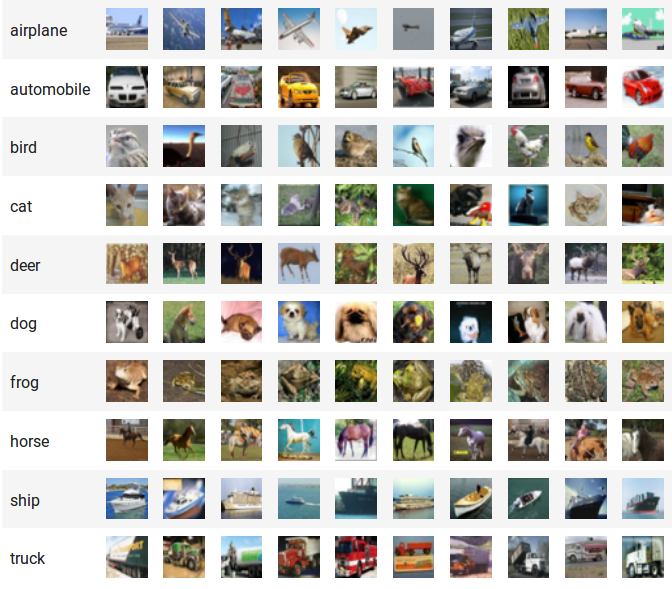
\includegraphics[scale=0.25]{cifar10.png}
\caption{Example images from the \cref{http://www.cs.toronto.edu/~kriz/cifar.html}{CIFAR-10} dataset.}
\end{figure}

\end{frame}

\section{Equations and Codes}
\subsection{Equations}
\begin{frame}
\frametitle{Equation Example}

\begin{block}{Some random equation:}
\begin{align*}
    \frac{\partial}{\partial \theta_k}J(\theta) 
        &= \frac{\partial}{\partial \theta_k}\Bigg[\frac{1}{m}\sum_{k=1}^m log(1+e^{-y^{(i)}\theta^Tx^{(i)}})\Bigg] \\
        &= \frac{1}{m}\sum_{k=1}^m \frac{1}{1+e^{-y^{(i)}\theta^Tx^{(i)}}}y^{(i)}x_k^{(i)} \\
        &= -\frac{1}{m}\sum_{k=1}^m h_\theta(-y^{(i)}x^{(i)})y^{(i)}x_k^{(i)}        
\end{align*}
\end{block}

\end{frame}


\subsection{Programming}
\begin{frame}[fragile]

\frametitle{Code Example \#1}

\begin{figure}
\centering
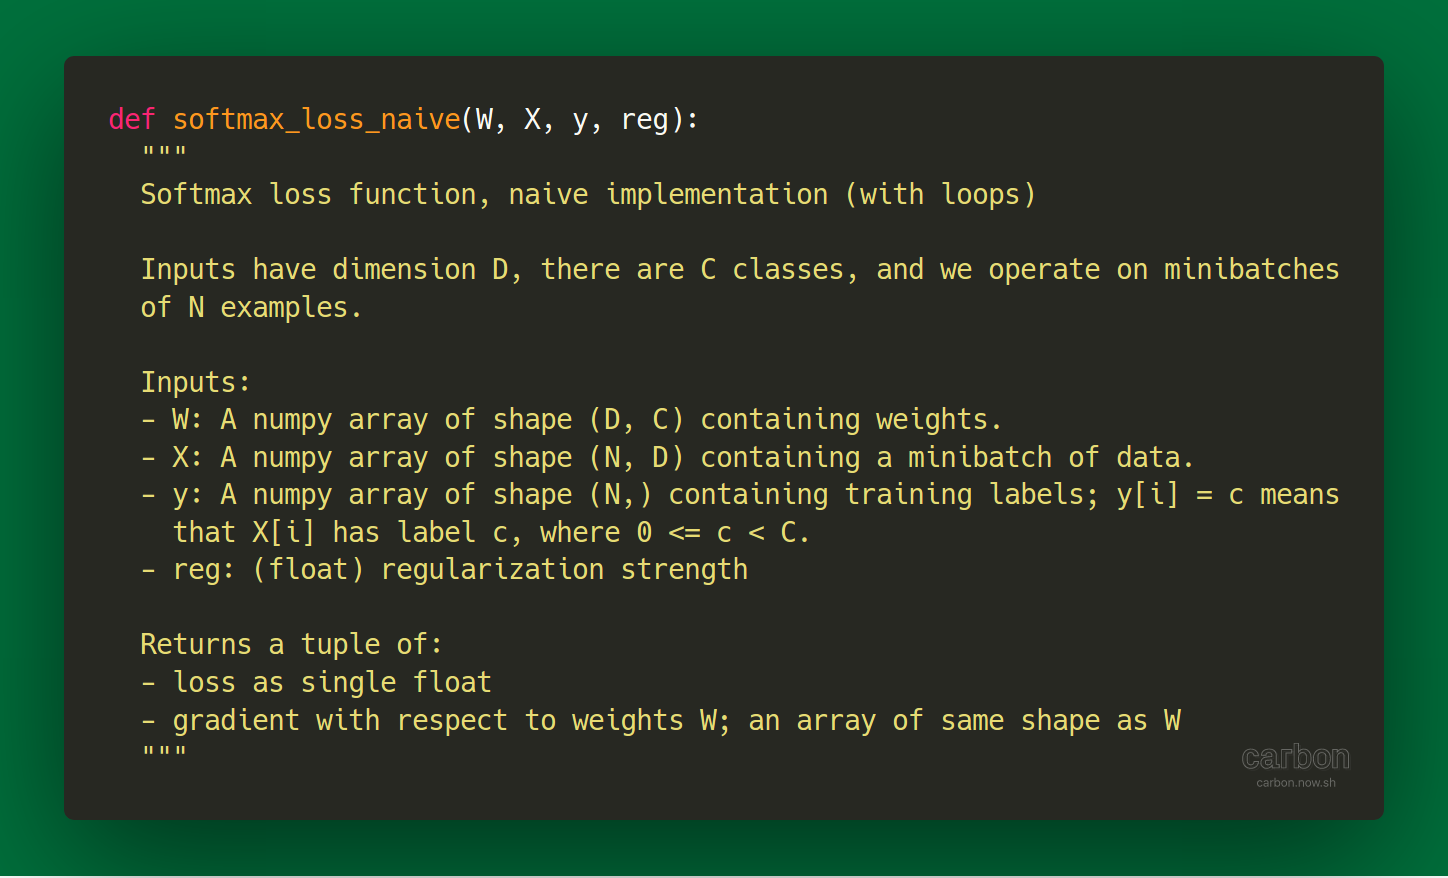
\includegraphics[width=\linewidth]{carbon.png}
\end{figure}
\blfootnote{\href{https://github.com/dawnlabs/carbon}{Carbon}}

\end{frame}

\begin{frame}[fragile]
\frametitle{Code Example \#2}

\code{\textbf{import} numpy \textbf{as} np}

\begin{lstlisting}[language=Python]
def code():
  # test comments #1    
  if True:
    for _ in range(5):
      print("Hello World 5 times")
  return None     
\end{lstlisting}

\end{frame}

\end{document}
